%\documentclass[handout]{beamer}
\documentclass{beamer}

\usepackage{xcolor}
\usepackage{hyperref}
\usepackage{amsmath}                   % \operatorname
\usepackage{amssymb}                   % \nexists
\usepackage{amsthm}
\usepackage{multicol}

\newtheorem{thm}{Theorem}

\usepackage{float}      % Allows for [H] positioning option in
\usepackage{subfigure}

\usepackage[export]{adjustbox}

\usepackage{fontawesome}

\usepackage{media9}

\usepackage{listings}
\lstset{basicstyle=\footnotesize}

\usepackage{tikz}
\usetikzlibrary{automata,shapes,arrows,positioning}
\usetikzlibrary{decorations.pathreplacing}

\usetikzlibrary{overlay-beamer-styles}

\tikzset{initial text={}}


\definecolor{uofstablue}{RGB}{0,83,155}
\definecolor{uofstalightblue}{RGB}{0,174,239}
\definecolor{uofstapurple}{RGB}{147,111,177}
\definecolor{uofstared}{RGB}{194,42,34}
\definecolor{uofstayellow}{RGB}{255,238,0}
\definecolor{uofstablack}{RGB}{0,0,0}
\definecolor{uofstaorange}{RGB}{248,152,29}
\definecolor{uofstaburgundy}{RGB}{139,18,51}
\definecolor{uofstagreen}{RGB}{120,194,64}
\definecolor{uofstagrey}{RGB}{113,112,116}
\definecolor{uofstadarkgreen}{RGB}{0,89,83}

\definecolor{uofstablueprint}{cmyk}{1,0.68,0,0.12}
\definecolor{uofstalightblueprint}{cmyk}{1,0,0,0}
\definecolor{uofstapurpleprint}{cmyk}{0.46,0.63,0,0}
\definecolor{uofstaredprint}{cmyk}{0,0.95,1,0}
\definecolor{uofstayellowprint}{cmyk}{0,0,1,0}
\definecolor{uofstablackprint}{cmyk}{0,0,0,1}
\definecolor{uofstaorangeprint}{cmyk}{0,0.48,1,0}
\definecolor{uofstaburgundyprint}{cmyk}{0,1,0.6,0.37}
\definecolor{uofstagreenprint}{cmyk}{0.69,0,1,0}
\definecolor{uofstagreyprint}{cmyk}{0,0.02,0,0.68}
\definecolor{uofstadarkgreenprint}{cmyk}{1,0,0.48,0.6}

% \definecolor{uofguniversityblue}{rgb}{0, 0.219608, 0.396078}
%
% \definecolor{uofgheather}{rgb}{0.356863, 0.32549, 0.490196}
% \definecolor{uofgaquamarine}{rgb}{0.603922, 0.72549, 0.678431}
% \definecolor{uofgslate}{rgb}{0.309804, 0.34902, 0.380392}
% \definecolor{uofgrose}{rgb}{0.823529, 0.470588, 0.709804}
% \definecolor{uofgmocha}{rgb}{0.709804, 0.564706, 0.47451}
% \definecolor{uofgsandstone}{rgb}{0.321569, 0.278431, 0.231373}
% \definecolor{uofgforest}{rgb}{0, 0.2, 0.129412}
% \definecolor{uofglawn}{rgb}{0.517647, 0.741176, 0}
% \definecolor{uofgcobalt}{rgb}{0, 0.615686, 0.92549}
% \definecolor{uofgturquoise}{rgb}{0, 0.709804, 0.819608}
% \definecolor{uofgsunshine}{rgb}{1.0, 0.862745, 0.211765}
% \definecolor{uofgpumpkin}{rgb}{1.0, 0.72549, 0.282353}
% \definecolor{uofgthistle}{rgb}{0.584314, 0.070588, 0.447059}
% \definecolor{uofgrust}{rgb}{0.603922, 0.227451, 0.023529}
% \definecolor{uofgburgundy}{rgb}{0.490196, 0.133333, 0.223529}
% \definecolor{uofgpillarbox}{rgb}{0.701961, 0.047059, 0}
% \definecolor{uofglavendar}{rgb}{0.356863, 0.301961, 0.580392}

%\tikzset{vertex/.style={draw, circle, inner sep=0pt, minimum size=0.5cm, font=\small\bfseries}}
%\tikzset{notvertex/.style={vertex, color=white, text=black}}
%\tikzset{plainvertex/.style={vertex}}
%\tikzset{vertexc1/.style={vertex, fill=uofgcobalt}}
%\tikzset{vertexc2/.style={vertex, fill=uofglawn}}
%\tikzset{vertexc3/.style={vertex, fill=uofgpumpkin}}
%\tikzset{vertexc4/.style={vertex, fill=uofgheather}}
%\tikzset{edge/.style={color=black!50!white}}
%\tikzset{bedge/.style={ultra thick}}
%\tikzset{edged/.style={color=screengrey, dashed}}
%\tikzset{edgel3/.style={color=uofgthistle, ultra thick}}

\newcommand*\circled[1]{\tikz[baseline=(char.base)]{
            \node[shape=circle,draw,inner sep=0pt] (char) {#1};}}

% {{{ theme things
\useoutertheme[footline=authortitle]{miniframes}
\useinnertheme{rectangles}

\setbeamerfont{block title}{size={}}
\setbeamerfont{title}{size=\Large,series=\bfseries}
\setbeamerfont{section title}{size=\large,series=\mdseries}
\setbeamerfont{author}{size=\large,series=\mdseries}
\setbeamercolor*{structure}{fg=uofstablue}
\setbeamercolor*{palette primary}{use=structure,fg=uofstablack,bg=white}
\setbeamercolor*{palette secondary}{use=structure,fg=white,bg=uofstalightblue}
\setbeamercolor*{palette tertiary}{use=structure,fg=white,bg=uofstablue}
\setbeamercolor*{palette quaternary}{fg=white,bg=uofstablack}

\setbeamercolor*{titlelike}{parent=palette primary}

\beamertemplatenavigationsymbolsempty

\setbeamertemplate{title page}
{
    \begin{tikzpicture}[remember picture, overlay]
        \node at (current page.north west) {
            \begin{tikzpicture}[remember picture, overlay]
                \fill [fill=uofstablue, anchor=north west] (0, 0) rectangle (\paperwidth, -2.6cm);
            \end{tikzpicture}
        };
        \node (logo) [anchor=north east, shift={(5.5cm,0cm)}] at (current page.north west) {
            
\includegraphics[keepaspectratio=true,scale=0.15]{../UniStALogos/03-standard-horizontal/02-standard-white.png}
        };
        % \node (logo) [anchor=north east, shift={(3cm,-5.5mm)}] at (current page.north) {
        %     \includegraphics[keepaspectratio=true,scale=0.56]{../OtherUniLogos/Victoria/UVic_hst_4c_cmyk.jpg}
        % };
        % \node (logo) [anchor=north east, shift={(-0.25cm,-0.55cm)}] at (current page.north east) {
        %     \includegraphics[keepaspectratio=true,scale=0.14]{../OtherUniLogos/VIXILogo/vixi-logo-expanded-large-bkg-white.png}
        % };
    \end{tikzpicture}
    \begin{tikzpicture}
        \node [anchor=west, xshift=0.2cm] at (current page.west) {
            \begin{minipage}{0.85\paperwidth}\raggedright
                \vskip 1.5cm
                {\usebeamerfont{title}\usebeamercolor[uofstadarkgreen]{}\inserttitle}\\[0.4cm]
                {\usebeamerfont{author}\usebeamercolor[uofstadarkgreen]{}\insertauthor}\\[0.3cm]
%                {\usebeamerfont{author}\usebeamercolor[uofstadarkgreen]{}\insertshortdate}\\[0.6cm]
                {\usebeamerfont{author}\usebeamercolor[uofstadarkgreen]{}\insertinstitute}
            \end{minipage}
        };
    \end{tikzpicture}
}

\setbeamertemplate{section page}
{
    \begin{centering}
        \begin{beamercolorbox}[sep=12pt,center]{part title}
            \usebeamerfont{section title}\insertsection\par
        \end{beamercolorbox}
    \end{centering}
}

\newcommand{\frameofframes}{/}
\newcommand{\setframeofframes}[1]{\renewcommand{\frameofframes}{#1}}

\makeatletter
\setbeamertemplate{footline}
{%
    \begin{beamercolorbox}[colsep=1.5pt]{upper separation line foot}
    \end{beamercolorbox}
    \begin{beamercolorbox}[ht=2.5ex,dp=1.125ex,%
        leftskip=.3cm,rightskip=.3cm plus1fil]{author in head/foot}%
        \leavevmode{\usebeamerfont{author in head/foot}\insertshortauthor}%
        \hfill%
        {\usebeamerfont{institute in head/foot}\usebeamercolor[fg]{institute in head/foot}\insertshortinstitute}%
    \end{beamercolorbox}%
    \begin{beamercolorbox}[ht=2.5ex,dp=1.125ex,%
        leftskip=.3cm,rightskip=.3cm plus1fil]{title in head/foot}%
        {\usebeamerfont{title in head/foot}\insertshorttitle}%
        \hfill%
        {\usebeamerfont{frame number}\usebeamercolor[fg]{frame number}\insertframenumber~\frameofframes~\inserttotalframenumber}
    \end{beamercolorbox}%
    \begin{beamercolorbox}[colsep=1.5pt]{lower separation line foot}
    \end{beamercolorbox}
}


\definecolor{dkgreen}{rgb}{0,0.6,0}
\definecolor{gray}{rgb}{0.5,0.5,0.5}
\definecolor{mauve}{rgb}{0.58,0,0.82}

\usepackage{listings}

\lstdefinelanguage{eprime}{
  keywords=[1]{forAll, letting, union, max, sum, exists, int, of, find, given, flatten, matrix, indexed, by, be, domain, ->, /\\, \\/, in, minimising, such, that, branching, on},
  keywordstyle=[1]\color{purple}\bfseries,
  keywords=[2]{atleast, atmost, gcc},
  keywordstyle=[2]\color{red}\bfseries,
  keywords=[3]{allDiff, toSet},
  keywordstyle=[3]\color{cyan}\bfseries,
  identifierstyle=\color{black},
  sensitive=false,
  comment=[l]{\$},
  commentstyle=\color{dkgreen}\ttfamily,
  stringstyle=\color{red}\ttfamily
}

\lstdefinelanguage{minizinc}{
  keywords=[1]{forall, constraint, [, ], false, function, if, in, else, or, and, solve, satisfy, then, include, predicate, endif, where, not, exists},
  keywordstyle=[1]\color{purple}\bfseries,
  keywords=[2]{int, set, of, true, false, bool, var, let, array, min, max},
  keywordstyle=[2]\color{blue}\bfseries,
  keywords=[3]{circuit, cumulative, regular, alldifferent, all_different, sum, all_equal, index_set, card, bool2int},
  keywordstyle=[3]\color{cyan}\bfseries,
  identifierstyle=\color{black},
  sensitive=false,
  comment=[l]{\%},
  commentstyle=\color{dkgreen}\ttfamily
}

\lstdefinestyle{mystyle}{
frame=tb,
aboveskip=3mm,
belowskip=3mm,
showstringspaces=false,
columns=flexible,
basicstyle={\small\ttfamily},
numbers=right,
numberstyle=\tiny\color{gray},
stringstyle=\color{mauve},
breaklines=true,
breakatwhitespace=true,
tabsize=3
}

\lstset{style=mystyle}



% }}}


\usepackage{algorithm}
%\usepackage{algorithmic} 
\usepackage[noend]{algpseudocode}

\title[Understanding Differences Between Modelling Pipelines]{Towards Understanding Differences Between Modelling Pipelines: a Modelers Perspective}
\author[R Hoffmann]{Csobán Balogh, \textbf{Ruth Hoffmann} and Joan Espasa}
\institute[ModRef 2024]{ModRef 2024, University of Girona}

\begin{document}

{
    \begin{frame}[plain,noframenumbering]
        \titlepage
    \end{frame}
}


\section*{Intro}
\begin{frame}{What and why?}
From a (single) users perspective:
    \begin{itemize}
        \item Investigate the capabilities of constraint programming pipelines.
        \item Investigate the difference in languages.
        \item Comparing MiniZinc and Savile Row.
    \end{itemize}
\end{frame}

\begin{frame}{How?}
\begin{itemize}
    \item Create as close to equivalent models as possible.
    \item Using MiniZinc and Essence' (not Essence)
    \item Compare over the same solver (Chuffed).
    \item Compare over equivalent(ish) optimisation levels.
    \item 6 Models from different problem classes
    \begin{enumerate}
        \item Quasigroup Completion, (no exciting differences)
        \item Wordpress Problem, (no exciting differences)
        \item Rotating Rostering Problem, (no exciting differences)
        \item Travelling Tournament Problem with Predefined Values, 
        \item Multi-Skilled Project Scheduling Problem,
        \item Capacitated Vehicle Routing Problem with Time Windows.
    \end{enumerate}
\end{itemize}
\end{frame}

\section*{Language Differences}
\begin{frame}{\texttt{regular} (MZn) vs \texttt{forAll} (SR)}
Traveling Tournament Problem with Predefined Venues at most three consecutive away or home games
\begin{itemize}
    \item at most three consecutive away or home games
    \item[MZn] \texttt{regular} asserts that a sequence of variables take a value from a finite automaton.
    \item[E'] \texttt{forAll} checking that there are not four consecutive assignments.
\end{itemize}
\end{frame}

\begin{frame}{\texttt{circuit} (MZn)}
Capacitated Vehicle Routing problem with Time Windows, Service Times and Pickup and Deliveries.
\begin{itemize}
    \item \texttt{circuit} is used to ensure the vehicle delivery routes do not take sub-tours in their route and visits each location uniquely for optimisation
    \item[MZn] A \texttt{circuit} is such that the cell value of an array points to the index of the next number, and this forms a circuit that continues around. 
    \item[E'] \url{https://github.com/MiniZinc/libminizinc/blob/master/share/minizinc/std/fzn_circuit.mzn}
\end{itemize}
\end{frame}


\begin{frame}{Set Variables}
    Multi-Skilled Project Scheduling Problem
    \begin{itemize}
        \item Sets of skills, workers etc. (each assigned an integer)
        \item[MZn] Variables which are a set.
        \item[E'] Occurrence representation of the integers/elements.
    \end{itemize} 
\end{frame}

\begin{frame}[containsverbatim]{\texttt{letting} (MZn)}
Multi-Skilled Project Scheduling Problem
\begin{itemize}
    \item \texttt{letting} creates variables within constraints
\end{itemize}
\begin{lstlisting}[basicstyle=\tiny, language=minizinc]
let { set of int: WTasks =
        { i | i in Tasks where  exists(k in has_skills[j])(rr[k, i] > 0) }
} in...
let { set of int: TWorkers = 
        { j | j in Workers where  exists(k in has_skills[j])(rr[k, i] > 0) }
} in...
\end{lstlisting}
\begin{lstlisting}[basicstyle=\tiny, language=eprime]
forAll i : Tasks . forAll j : Workers .
    TWorkers[j, i] = 1 <-> 
        exists k : Skills . has_skills[j, k] = 1 /\ rr[k,i] > 0,
\end{lstlisting}
\end{frame}


\begin{frame}{\texttt{cumulative} (MZn)}
Multi-Skilled Project Scheduling Problem
\begin{itemize}
    \item Determines whether set of tasks with start times, durations, and resource requirements, never exceed the global resource bound at any time.
    \item[MZn] Determines if a cumulative resource usage is within bounds.
    \item[E'] \url{https://github.com/MiniZinc/libminizinc/blob/master/share/minizinc/std/fzn_cumulative.mzn}
\end{itemize}
\end{frame}

\section*{Results}
\begin{frame}{Results}
{\footnotesize{

\begin{table}[h!]
    \centering
    \begin{tabular}{c|c|ccc|ccc}
    & & \multicolumn{3}{c|}{E'} & \multicolumn{3}{c}{MZn} \\
    Problem & \# & O0S0 & O2S1 & O3S2 & O0 & O1 & O5 \\ \hline
    Quasigroup           & 43 & 41 & 42 & 41 & 40 & 39 & 40 \\        
    Quasigroup Occ.      & 43 & 41 & 41 & 42 & 32 & 37 & 38 \\
    Wordpress            & 9  & 6  & 6  & 6  & 6  & 6  & 6  \\               
    Wordpress Symm.      & 9  & 4  & 4  & 6  & 4  & 4  & 4  \\ 
    TTPPV                & 20 & 3  & 3  & 3  & 3  & 3  & 3  \\ 
    MSPSP                & 6  & 6  & 6  & 6  & 6  & 6  & 6  \\ 
    CVRPTW               & 5  & 0  & 0  & 0  & 0  & 0  & 0  \\ 
    Rostering            & 7  & 7  & 7  & 7  & 7  & 7  & 7    
    \end{tabular}
\end{table}}}
\end{frame}

\begin{frame}
\begin{center}
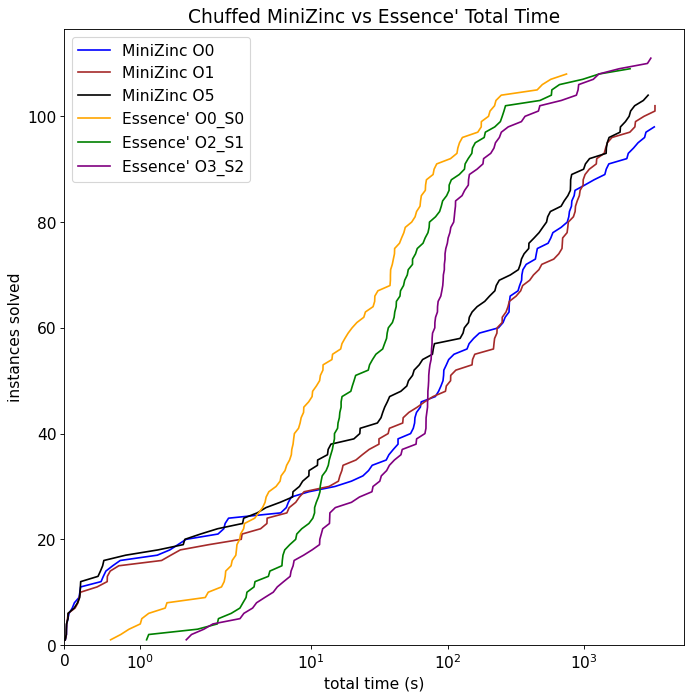
\includegraphics[scale=0.3]{../python/graphs/paper_total_cactus.png}
\end{center}
\end{frame}

\section*{Take Away}
\begin{frame}{Take Away}
\begin{itemize}
    \item[MZn] allows better (expert) modeler control
    \item[MZn] provides a slightly more expressive language due to the facilities for code organization and reusability
    \item[SR] provides a solid set of default settings
    \item[SR] has a more consistent performance profile
\end{itemize}    

\end{frame}

\section*{}
\begin{frame}[plain,noframenumbering,b]
    \begin{tikzpicture}[remember picture, overlay]
        \node at (current page.north west) {
            \begin{tikzpicture}[remember picture, overlay]
                \fill [fill=uofstablue, anchor=north west] (0, 0) rectangle (\paperwidth, -1.7cm);
            \end{tikzpicture}
        };

        \node (logo) [anchor=north east, shift={(-0.1cm,0.2cm)}] at (current page.north east) {
            
\includegraphics[keepaspectratio=true,scale=0.12]{UniStALogos/03-standard-horizontal/02-standard-white.png}
        };
    \end{tikzpicture}

    \begin{center}
        {\Large{Thank you!}} \\ \vspace{1cm}
        \href{https://github.com/ruthhoffmann}{ \faGithub\ ruthhoffmann} \\ [2mm]
        \href{https://www.st-andrews.ac.uk/computer-science/people/rh347/}{ \faDesktop\ www.st-andrews.ac.uk/computer-science/people/rh347/} \\ [2mm]
        \href{mailto:rh347@st-andrews.ac.uk}{\faEnvelope\ \nolinkurl{rh347@st-andrews.ac.uk}} \\ [1cm]
        %Find me in my office \\ [1cm]
    \end{center}
\end{frame}

\end{document}
